\documentclass{beamer}
\usepackage[utf8]{inputenc}

\let\svthefootnote\thefootnote

% links
\usepackage{hyperref}
\usepackage{nameref}
% figures with tikz
\usepackage{tikz,pgf,pgfplotstable} % tikz package 
\usetikzlibrary{arrows.meta,
                backgrounds,
                calc, chains, 
                fit,
                patterns,
                positioning,
                shapes,}
\usepackage{lmodern}
% font personalization 
\usepackage{transparent}
\usepackage{verbatim}
\newcommand{\semitransp}[2][40]{\textcolor{fg!#1}{#2}}
\usepackage[super]{nth}
\usepackage{listings}
\usepackage{booktabs}
\usepackage[absolute,overlay]{textpos}
\usepackage{xcolor}
\usepackage{latexsym,xcolor,multicol,booktabs,calligra}
\usepackage{amsmath,amssymb,BOONDOX-cal,bm}	
\usepackage{pstricks}
\usepackage{stackengine}   
\usepackage{graphicx}
\graphicspath{{figures/}}
\usepackage{romannum}
\usepackage{minted}
% deleting lower navigation symbols in slides
\setbeamertemplate{navigation symbols}{}
% reference setup
\usepackage[natbib=true,style=alphabetic-verb,backend=bibtex,useprefix=true]{biblatex}
\addbibresource{biblio.bib}

% title setup
\author{\textbf{Antonio Pucciarelli}}
\title{\textsc{Turbomachinery: Compressor preliminary design}}
\institute{Politecnico di Milano} 
\date{\today}
\logo{\includegraphics[width=0.2\textwidth]{polimiLogo.jpeg}}
\newcommand{\nologo}{\setbeamertemplate{logo}{}}

% slide decoration package
\usepackage{Wue}
\newtheorem{thm}{Theorem}[theorem]

% color personalization
\def\cmd#1{\texttt{\color{red}\footnotesize $\backslash$#1}}
\def\env#1{\texttt{\color{blue}\footnotesize #1}}
\definecolor{mygreen}{rgb}{0,0.6,0}
\definecolor{mygray}{rgb}{0.5,0.5,0.5}
\definecolor{mymauve}{rgb}{0.58,0,0.82}
\definecolor{codegreen}{rgb}{0,0.6,0}
\definecolor{codegray}{rgb}{0.5,0.5,0.5}
\definecolor{codepurple}{rgb}{0.58,0,0.82}
\definecolor{backcolour}{rgb}{0.95,0.95,0.92}
\definecolor{LightGray}{gray}{0.9}

\begin{document}
	\begin{frame}
		\titlepage
    \end{frame}

	\section{Problem Description}
        \begin{frame}{Initial conditions \& constraints}
	\begin{block}{Inlet conditions}
		\begin{itemize}
			\item $P_{T0} = 1 bar$
			\item $T_{T0} = 300 K$
		\end{itemize}
	\end{block}
	\begin{alertblock}{Constraints}
		\begin{itemize}
			\item $r_{max} = 0.45 m$
			\item $\beta_{TT} = 1.45$
			\item $\dot{m} = 100 \frac{kg}{s}$
			\item \textbf{max} $\eta$
		\end{itemize}
	\end{alertblock}
	Due to the \textbf{course track} and \textbf{preference}, the turbomachinery design will be on an \textbf{axial} compressor.
\end{frame}

        
	\section{Mean Line}
        \subsection{Problem setup}
	{\nologo
	\begin{frame}{Problem setup: hypothesis}
		\begin{alertblock}{Hypothesis}
			\begin{itemize}
				\item \textbf{not using} an \textbf{inlet guide vane} for simplicity of design
				\item keeping, in the similarity/adimensional analysis of the compressor, $V_{a_{mean}}$ \textbf{constant}\footnote{$\dot{m}$ corrections will be made later on in the \textbf{radial equilibrium} solution.}  
				\item keeping the blade height, $b_0$, \textbf{constant} both in rotor and stator
				\item using a \textbf{mixed vortex} model for the \textbf{rotor} velocity triangles
				\item using a \textbf{second order} function for the \textbf{stator} velocity triangles 
				\item neglecting inlet \textbf{entropy} generation and assuming \textbf{rotor inlet} quantities \textbf{constant}
				\item \textbf{shrouding} at blade tip not present
				\item \textbf{rotor-stator} losses neglected
			\end{itemize}
		\end{alertblock}
	\end{frame}
	}
	
	\begin{frame}{Problem setup: solution steps}
		\begin{block}{Main procedural steps:}
			\begin{itemize}
				\item $\lambda$ and $\psi$ computation from $\chi$ and $V_{t0}$
				\item $\phi$ and $\eta$ computation 
				\item $V_{a_{mean}}$ and $L_{eu}$ computation from $\phi$, $\beta_{TT}$ and $\eta$
				\item computing \textbf{mean} velocity triangles, using the above hypothesis
				\item computing \textbf{mean thermodynamic} quantities 
				\item computing \textbf{blade height}
			\end{itemize}
		\end{block}
	\end{frame}

\subsection{Main design quantities}
	{\nologo
	\begin{frame}{Graph analysis: $\chi$ \& $r_{mean}$}
		\begin{figure}
			\centering
			\includegraphics[width=\textwidth]{figures/rMeanChi.pdf}
		\end{figure}
	\end{frame}	

	\begin{frame}{Graph analysis: \textbf{rotor} $\alpha$, $\beta$ \& $V_{t}$}
		\begin{figure}
			\centering
			\includegraphics[width=\textwidth]{figures/betaAngles.pdf}
		\end{figure}
	\end{frame}
	
	\begin{frame}{Graph analysis: \textbf{stator} $\alpha$ \& $V_{t}$}
		\begin{figure}
			\centering
			\includegraphics[width=\textwidth]{figures/alphaAngles.pdf}
		\end{figure}
	\end{frame}
	}

	\begin{frame}{$\lambda$ \& $\psi$}
		From the previous \textbf{graphs}:
		\begin{itemize}
            \item \let\thefootnote\relax\footnotetext{\vspace{0.2cm}$\chi = \frac{h_1 - h_0}{h_{T1} - h_{T0}} = \frac{\frac{W_0^2}{2} - \frac{W_1^2}{2}}{U_{mean} (V_{t1} - V_{t0})} = \frac{\frac{W_{a0}^2}{2} + \frac{W_{t0}^2}{2}- \frac{W_{a1}^2}{2} - \frac{W_{t1}^2}{2}}{U_{mean} (V_{t1} - V_{t0})} = \frac{\frac{W_{t0}^2}{2} - \frac{W_{t1}^2}{2}}{U_{mean} (V_{t1} - V_{t0})}.$}$\chi = 0.58$
				  \let\thefootnote\svthefootnote
			\item $r_{mean} = 0.32 m$
			\item $\frac{V_{t0}}{U_{mean}} = 0$
		\end{itemize}
		Taking into account the previous modeling \textbf{hypothesis}:
		\begin{align}
			\lambda & = \Bigg( 1 - \chi - \frac{V_{t0}}{U_{mean}} \Bigg) \cdot 4 \nonumber \\
			\psi    & = \frac{\lambda}{2} = \frac{L_{eu_{mean}}}{U_{mean}^2} \nonumber
		\end{align}
	\end{frame}
	
	\begin{frame}{$\phi_{(\psi)}$}
		From \cite[Sec. 10.4]{axial2004} it is imposed that $\frac{W_2}{W_1} \geq 0.7$ with a \textit{safety} margin of $3 \%$. $\phi_{lim}$ line\let\thefootnote\relax\footnotetext{$\phi = \frac{V_{a_{mean}}}{U_{mean}}$.\vspace{1cm}} \let\thefootnote\svthefootnote is related to the \textbf{surge safety margin}.  
		\begin{figure}
			\centering
			\includegraphics[width=0.7\textwidth]{figures/stagePerf.pdf}
		\end{figure}
	\end{frame}

	\begin{frame}{$\eta$ \& $L_{eu}$}
		$\eta$ is computed from an \textbf{Lieblein} efficiency chart\footnote{This chart has been interpolated from the course slides charts.} given $\phi$ and $\chi$. This parameter will be used for the computation of $L_{eu}$ given the $\beta_{TT}$ target.
		\begin{columns}
			\column{0.5\textwidth}
				\begin{figure}
					\centering 
					\includegraphics[width=1\textwidth]{figures/efficiency.pdf}
				\end{figure}
			\column{0.5\textwidth}
			\begin{align}
				L_{is} & = \frac{\gamma \ R}{\gamma - 1} \ T_{T0} \ (\beta_{TT}^{{\frac{\gamma - 1}{\gamma}}} - 1) \nonumber \\
				L_{eu} & = \frac{L_{is}}{\eta} \nonumber
			\end{align}
		\end{columns}
	\end{frame}

	\subsection{$V_{t_{mean}}$, $V_{a_{mean}}$, $U_{mean}$ \& velocity triangles}
\begin{frame}[fragile]{$V_{a_{mean}}$, $V_{t_{mean}}$ \& $U_{mean}$}
	\vspace{-0.8cm}
	\begin{align}
		U_{mean}      & = \sqrt{\frac{L_{eu_{mean}}}{\psi}} \nonumber \\ 
		V_{a_{mean}}  & = \phi \ U_{mean} \nonumber \\
		L_{eu_{mean}} & = U_{1_{mean}} \ V_{t1_{mean}} - U_{0_{mean}} \ V_{t0_{mean}} \overset{U_1 = U_0}{=} U_{mean} \ \Delta V_{t_{mean}} \nonumber \\
		V_{t1_{mean}} & = \Delta V_{t_{mean}} + V_{t0_{mean}} \nonumber  
	\end{align}
	\vspace{-0.3cm}
	\begin{itemize}
		\item $\Delta V_{t_{mean}}$ computation allows us to get a \textit{first sketch} of the \textbf{velocity triangles}\footnote{\textbf{Mixed vortex} model and \textbf{second order} function based.} using $\phi$, $\psi$ and $L_{eu}$\footnote{$L_{eu} = U_1 \ V_{t1} - U_0 \ V_{t0}$.} definitions. $V_a$ is assumed \textbf{constant} all through the stage
		\item The first analysis results are stored in \verb|compressor_0.58_0.32_45_35.txt|
	\end{itemize}
\end{frame}

%\begin{frame}{Nomenclature}
%    \scriptsize{
%        \begin{itemize}
%            \item $\mathtt{0, 1, 2}$: rotor inlet, rotor outlet/stator inlet, stator outlet
%            \item $P_{T0}$: inlet total pressure 
%            \item $T_{T0}$: inlet total temperature
%            \item $r_{max}$: max rotor/stator tip radius
%            \item $\beta_{TT}$: pressure ratio expressed in total pressure 
%            \item $\dot{m}$: mass flux 
%            \item $\eta$: efficiency
%            \item $\psi$: stage work coefficient
%            \item $\phi$: stage flow coefficient 
%            \item $\chi$: reaction degree 
%            \item $\omega$: rotation speed 
%            \item $V_{*}$: absolute speed at $\mathtt{*}$ station
%            \item $V_{a*}$: axial absolute speed at $\mathtt{*}$ station
%            \item $V_{t*}$: tangential absolute speed at $\mathtt{*}$ station 
%            \item $W_{*}$: relative speed at $\mathtt{*}$ station
%            \item $W_{a*}$: axial relative speed at $\mathtt{*}$ station
%            \item $W_{t*}$: tangential relative speed at $\mathtt{*}$ station 
%            \item $L_{is}$: isentropic work 
%            \item $L_{eu}$: real work 
%            \item $U_{mean}$: rotational speed at meanline 
%            \item $\gamma$: specific heat ratio 
%            \item $R$: gas constant
%        \end{itemize}
%    }
%\end{frame}

    
   	\section{Models}
        \subsection{Losses modeling} \label{lossesModeling}
\subsubsection{Profile losses}
	{\nologo
	\begin{frame}{Profile losses}
		The profile losses used are related to the \textbf{Leiblein modeling} approach\footnote{The following equations are interpolated data from \cite[Sec. 6.4]{axial2004}.}.
		\newline
		The model is based on the \textbf{equivalent diffusion factor}\footnote{It describes how important is the \textbf{velocity change} along the blade. It can be seen as an \textit{indicator} of the \textbf{blade loading}.}, $D_{eq}$:
		\begin{align}
			\frac{W_{max}}{W_1} & = 1.12 + 0.61 \ \frac{cos(\beta_1)^2}{\sigma} \cdot \frac{r_1 \ V_{t1} - r_2 \ V_{t2}}{r_1 \ V_{a1}} \nonumber \\
			D_{eq} & = \frac{W_{max}}{W_1} \cdot \frac{W_1}{W_2} \nonumber  
		\end{align}
		$D_{eq}$ will be used for the computation of $\bar{\omega}_{profile}$ as:
		\begin{equation}
			\bar{\omega}_{profile} = \frac{0.004 \ \Big( 1 + 3.1 \ \big( D_{eq} - 1 \big)^2 + 0.4 \ \big( D_{eq} - 1 \big)^8 \Big) \ 2 \ \sigma}{cos(\beta_2) \ \Big( \frac{W_1}{W_2} \Big)^2} \nonumber
		\end{equation}
	\end{frame}
	}

\subsubsection{Compressibility losses}
	{\nologo
	\begin{frame}{Compressibility losses -- \Romannum{1}}
		 These losses can be seen as a \textbf{correction} of the \textbf{profile} losses due to the compressibility of the gas along its \textit{journey} in the stage. 
		 \newline
		 \newline
		 The correction refers to a \textbf{Leiblein correction} model that uses the \textbf{positive} and \textbf{negative} blade section incidence angle\footnote{$i_c$ and $i_s$ are related to the total pressure losses, $\bar{\omega}_c$ and $\bar{\omega}_s$, that are \textbf{twice} the minimum total pressure loss, $\bar{\omega}$, obtained at the \textbf{design incidence angle}, $i^*$.}, $i_c$ and $i_s$. 
		 \newline
		 \newline
		 These new stall incidence angles will build a new \textbf{mean} incidence angle, $i_m$, that can be seen as the \textbf{optimum} incidence angle related to the inlet Mach conditions\footnote{The implemented model follows \cite[Sec. 6.6]{axial2004}.}. 
	\end{frame}
	}
	\begin{frame}{Compressibility losses -- \Romannum{2}}
		$\bar{\omega}_{compressibility}$ setup:
		\begin{itemize}
			\item $R_c$ and $R_s$ computation\footnote{$R_{c}$ and $R_{s}$ are \textbf{range indices} for the computation of $i_c$ and $i_s$.}:
				\begin{align}
					R_c & = 9 - \Bigg[1 - \Bigg( \frac{30}{\beta_1} \Bigg)^{0.48} \Bigg] \ \frac{\theta}{8.2} \nonumber \\
					R_s & = 10.3 + \Bigg( 2.92 - \frac{\beta_1}{15.6} \Bigg) \ \frac{\theta}{8.2} \nonumber  
				\end{align}
			\item $i_c$ and $i_s$ computation due to \textbf{compressibility} effects:
				\begin{align}
					i_c & = i^{*} - \frac{R_c}{1 + 0.5 \ M_{1}^{3}} \nonumber \\
					i_s & = i^{*} + \frac{R_s}{1 + 0.5 \Big( K_{sh} \ M_{1} \Big)^3} \nonumber 
				\end{align}
		\end{itemize}
	\end{frame}

	{\nologo
	\begin{frame}{Compressibility losses -- \Romannum{3}}
		\begin{itemize}
			\item $i_m$ computation\footnote{$i_m$ is the incidence angle at wich corresponds, having accounted the \textbf{compressibility}, the \textbf{minimum pressure loss}, $\bar{\omega}_m$.}: $i_m = i_c + \Big( i_s - i_c \Big) \ \frac{R_c}{R_c + R_s}$
			\item $\bar{\omega}_{m}$ computation: $\bar{\omega}_{m} = \bar{\omega}_{profile} \ \Bigg[ 1 + \frac{\big( i_m - i^{*} \big)^2}{R_s^{2}} \Bigg]$
			\item $\bar{\omega}_{compressibility}$ computation\footnote{After having computed $i_c$, $i_s$, $i_m$ and $\bar{\omega}_m$. $\bar{\omega}_{compressibility}$ is a function of $i$. In the \textbf{total pressure losses study}: $\bar{\omega}_{compressibility} = \bar{\omega}_{compressibility_{(i^*)}}$.}: 
				\begin{align}
					\bar{\omega}_{compressibility} = \bar{\omega}_m + \bar{\omega}_m \ \Bigg[ \frac{i - i_m}{i_c - i_m} \Bigg]^2 \text{, if } i \leq i_m\nonumber \\ 
					\bar{\omega}_{compressibility} = \bar{\omega}_m + \bar{\omega}_m \ \Bigg[ \frac{i - i_m}{i_s - i_m} \Bigg]^2 \text{, if } i \geq i_m \nonumber 
				\end{align}
		\end{itemize}
	\end{frame}
	}

\subsubsection{Secondary flow losses}
	\begin{frame}{Secondary flow losses}
		These losses are relative to the \textbf{secondary flow} inside the compressor and are \textit{usually} \textbf{greater} than the other losses. These losses are related to \textbf{eddies} generated with the \textbf{blade-flow} interaction and \textbf{streamlines} displacement due to the presence of \textbf{pressure gradients}. 
		\newline 
		These losses are computed with \textbf{Howell}'s model \cite[Ch. 6]{axial2004}\footnote{Howell computed a secondary flow loss model that is automatically embedded into $\bar{\omega}_{profile}$. It is used for the \textbf{estimation} of the \textbf{blade number}.}:
		\begin{align}
			\bar{\beta} & = \frac{arctan( tan( \beta_1 ) + tan( \beta_2 ) )}{2}; & \text{\Romannum{1}} \nonumber \\ 
			C_{L} & = 2 \ cos( \bar{\beta} ) \cdot \frac{tan( \beta_1 ) - tan( \beta_2 )}{\sigma}; & \text{\Romannum{2}} \nonumber \\
			C_{D} & = 0.18 \ C_{L}^2; & \text{\Romannum{3}} \nonumber \\
			\bar{\omega}_{secondary} & = C_{D} \ \sigma \cdot \frac{cos( \beta_1 )^2}{cos( \bar{\beta} )^3}; & \text{loss computation} \nonumber 
		\end{align}
	\end{frame}

\subsubsection{End wall losses}
	\begin{frame}{End wall losses}
		These losses are related the interaction between the flow and the \textbf{compressor case}. They are \textit{lower} than the \textbf{secondary flow} losses.
		\newline
		It has been used a simple and fast relation made by \textbf{Howell} \cite[Ch. 6]{axial2004}\footnote{This loss is kept into account in the \textbf{blade numbering} study.}:
		\begin{align}
			C_{D} & = 0.02 \ \frac{s}{b_{0}} \nonumber \\ 
			\bar{\omega}_{endWall} & = C_{D} \ \sigma \cdot \frac{cos( \beta_1 )^2}{cos( \bar{\beta} )^3}; & \text{loss computation} \nonumber 
		\end{align}		
	\end{frame}

\subsubsection{Shock losses}
	\begin{frame}{Shock losses -- \Romannum{1}}
		The \textbf{relative} Mach number at the rotor inlet is slightly above \textbf{sonic speed}; a \textbf{shock wave} will be present at the rotor tip. From \cite{manfredi2020transonic}, \textbf{shock pattern} is related to \textbf{Mach number} and \textbf{airfoil shape}.
		\newline
		\newline 
		The \textbf{shock} losses modeling is related to \textbf{K\"onig losses} modeling approach. This model describes a \textbf{2 shock waves loss}\footnote{For a flow in \textbf{unstarted condition}: shock wave \textit{followed by} an expansion wave and another shock wave. \textbf{Unstarted conditions} are for $M_{a,r} < 1$.} using a \textbf{single normal shock} with respect to a computed Mach number, $M_{in}$. 
		\newline
		\newline
		\textbf{K\"onig model} depends mainly on \textbf{blade deflection angle}, $\theta$, and \textbf{relative inlet Mach}\footnote{\textbf{Leading edge radius} is not taken into account due to the \\ \textit{approximated nature} of the model.}, $M_{1,r}$.
	\end{frame}
	
	\begin{frame}{Shock losses -- \Romannum{2}}
		\textbf{Swan} and \textbf{Miller}, \cite[Sec. 6.7]{axial2004}, derived a \textbf{shock loss formulation} from \textbf{K\"onig model}. 
		\newline 
		\newline
		The following are the steps made for the computation of the \textbf{shock loss}, $\bar{\omega}_{shock}$, at each \textbf{blade section}:
		\begin{itemize}
			\item computation of the \textbf{expansion wave} angle, $\phi$: 
				\begin{equation}
					\phi = \frac{s \ cos(\psi)}{s \ sin(\psi) \ R_u}; \text{ where } \psi = \psi_{(\beta_1, \ \gamma, \ \theta)} \nonumber
				\end{equation}
			\item computation of $W_s$ and $M_s$ using \textbf{Prandtl-Meyer} expansion: 
			\begin{equation}
				\phi = \int_{W_1}^{W_s} \sqrt{M^2 - 1} \ \frac{dW}{W} \nonumber
			\end{equation}
			\item $M_{in}$ computation: $M_{in} = \sqrt{M_{1,r} \ M_s}$
			\item \textbf{normal shock} solution and computation of $\Delta P_T$
			\item from $\Delta P_T$, computation of $\bar{\omega}_{shock}$
		\end{itemize}
	\end{frame}

\subsubsection{Tip leackage losses}
	{\nologo
	\begin{frame}{Tip leackage losses}
		Again these losses are computed from \cite[Sec. 6.9]{axial2004}. The main concept is: computing a \textbf{total} blade pressure loss and \textbf{assuming linear distribution} of losses from the hub to the tip\footnote{$Z$ is the number of blades. $\delta_c$ is the tip clearance. $N_{row}$ is the number of blade rows in the compressor.}. 
		\begin{align}
			\tau & = \pi \ \delta_c \Big[ r_1 \rho_1 V_{a1_{mean}} + r_2 \rho_2 V_{a2_{mean}} \Big] \Big[ r_2 V_{t2_{mean}} - r_1 V_{t1_{mean}} \Big] \nonumber \\ 
			\Delta P & = \frac{\tau}{Z \ r_{tip} \delta_c \ c \ cos(\gamma)} \nonumber \\ 
			U_c & = 0.816 \frac{\sqrt{\frac{2 \Delta P}{\rho_{mean}}}}{N_{row}^{0.2}} \nonumber \\ 
			\dot{m_c} & = \rho_{mean} \ U_c \ Z \ \delta_c \ c \ cos(\gamma) \nonumber \\ 
			\Delta P_T & = \frac{\Delta P \ \dot{m_c}}{\dot{m}} \nonumber  
		\end{align}
		$\Delta P_T$ is the \textbf{overall} total pressure loss due to \textbf{tip leackage}.
		\vspace{0.11cm}
	\end{frame}
	}

\subsection{Blade shape}
	{\nologo
	\begin{frame}{Blade shape setup}
		The \textbf{Leiblein model} from \cite[Ch. 6]{axial2004} has been used for the blade shape computation. 
		\newline 
		\newline
		$\mathtt{NACA-65}$ profile has been chosen for the blade generation\footnote{Due to the low tip sonic Mach number it has been chosen to use this profile as well for the blade tip instead of a supersonic adapted profile shape.}.
		\newline
		\newline
		The \textbf{main contraints} are: $\frac{t_b}{c} \approx 0.1$ and $\sigma$ is related just to $s$\footnote{$\frac{t_b}{c} \approx 0.1$ allows setting $K_{sh} \approx 0.1$. The blade chord, $c$, is set up as constant during the \textbf{blade numbering} study: using $AR = \frac{b_0}{c}$.}.
		\newline
		\newline
		Due to the many possible blade configurations, an \textbf{optimization} procedure has been used for the computation of $i^{*}$, $\delta$ and $\theta$. 
		\newline
		\newline
		Each section airfoil shape is \textbf{computed} from $\theta$ and $\mathtt{NACA-65} \ C_{L0}$ surface coordinates.
	\end{frame}
	}

	\begin{frame}{$i^*$ computation}
		The \textbf{incidence angle}, $i^*$, is computed using:
		\begin{align}
			K_{t,i} & = \Bigg( 10 \ \frac{t_b}{c} \Bigg)^q \ \text{; where} \ q = \frac{0.28}{0.1 + (\frac{t_b}{c})^{0.3}} \nonumber \\ 
			(i^*_0)_{10} & = \frac{\beta_0^p}{5 + 46 \cdot e^{-2.3 \sigma}} - 0.1 \ \sigma^{3} \ e^{\frac{\beta_0 - 70}{4}} \ \text{; where} \ p = 0.914 + \frac{\sigma^3}{160} \nonumber \\
			n & = 0.025 \sigma - 0.06 - \frac{\Big(\frac{\beta_0}{90} \Big)^{1 + 1.2 \sigma}}{1.5 + 0.43 \sigma} \nonumber \\ 
			i^* & = K_{sh} \ K_{t,i} \ (i^*_0)_{10} + n \ \theta \nonumber 
		\end{align}
	\end{frame}

	\begin{frame}{$\delta$ computation}
		The \textbf{deviation angle}, $\delta$, is computed using:
		\begin{align}
			K_{t,\delta} & = 6.25 \frac{t_b}{c} + 37.5 \Bigg(\frac{t_b}{c}\Bigg)^2 \nonumber \\ 
			(\delta^*_0)_{10} & = 0.01 \sigma \beta_0 + (0.74 \sigma^{1.9} + 3 \sigma) \Bigg(\frac{\beta_0}{90}\Bigg)^{1.67 + 1.09 \sigma} \nonumber \\
			b & = 0.9625 - 0.17 \frac{\beta_0}{100} - 0.85 \Bigg(\frac{\beta_0}{100}\Bigg)^3 \nonumber \\ 
			m & = \frac{m_{1.0}}{\sigma^b} \ \text{; where} \ m_{1.0} = 0.17 - 0.0333 \frac{\beta_0}{100} + 0.333 \Bigg(\frac{\beta_0}{100}\Bigg)^2 \nonumber \\
			\delta & = K_{sh} \ K_{t,\delta} \ (\delta^*_0)_{10} + m \ \theta \nonumber  
		\end{align}
	\end{frame}

	\begin{frame}{$\theta$ computation}
		Starting from the \textbf{known} flow deflection angle\footnote{$\varepsilon = \beta_{inlet} - \beta_{outlet}$. $\beta_1$ and $\beta_2$ change with respect to the \textbf{axial speed}.}, $\varepsilon$, it is necessary to compute:
		\begin{equation}
			\theta = \varepsilon - i^* + \delta \nonumber
		\end{equation}
		Since $i^*$ and $\delta$ are functions of $\theta$, the computation of $\theta$ is made by an \textbf{iterative process}:
		\begin{equation}
			\theta = \varepsilon - i^*_{(\theta)} + \delta_{(\theta)} \nonumber
		\end{equation}
		Once found $\theta$, the \textbf{total pressure loss} coefficients, $\bar{\omega}_{*}$, are computed.   
	\end{frame}

\subsection{Radial equilibrium}
	\begin{frame}{Equation setup}
		The \textbf{radial equilibrium} equation: $\frac{\partial h_t}{\partial r} = T \frac{\partial s}{\partial r} + V_a \frac{\partial V_a}{\partial r} + V_t \frac{\partial r V_t}{\partial r}$ is converted into, for the exit station\footnote{$1$ is the blade inlet station and $2$ is the blade outlet section.} of the blade, a \textbf{1st order ODE}:
		\begin{equation}
			\begin{split}
				- \frac{1}{2} \frac{\partial V_{a2}^2}{\partial r} + \frac{V_{a2}^2}{2 \ c_P} \frac{\partial s_{2}}{\partial r} = - c_P \frac{\partial T_{T1}}{\partial r} - \omega \ \frac{\partial r V_{t2}}{\partial r} + \omega \ \frac{\partial r V_{t1}}{\partial r} \\ + T_{T1} \ \frac{\partial s_2}{\partial r} + \frac{\omega}{c_P} r V_{t2} \ \frac{\partial s_2}{\partial r} - \frac{\omega}{c_P} r V_{t1} \frac{\partial s_2}{\partial r} - \frac{1}{2 \ c_P} V_{t2}^2 \frac{\partial s_2}{\partial r} + \frac{V_{t2}}{r} \frac{\partial r V_{t2}}{\partial r}	
			\nonumber
			\end{split}
		\end{equation}
		\begin{itemize}
			\item The \textbf{ODE} will be solved for $V_{a2}^2$ 
			\item $s_2$ is computed from\footnote{$\bar{\omega}_{*}$ computation has been treated earlier in \hyperlink{lossesModeling}{{\color{blue} \nameref{lossesModeling}}}.} $\sum_i \bar{\omega}_{i}$
			\item $\omega, V_{t1}, V_{t2} \ \text{and} \ T_{T1}$ are known
		\end{itemize}
	\end{frame}
	
	\begin{frame}{$\Delta s$ computation}
		From pressure loss coefficients it is possible compute the \textbf{outlet total pressure} as: 
		\begin{equation}
			P_{T2,r} = P_{T1,r} + \sum_i \bar{\omega}_{i} \ (P_{T1,r} - P_{1,r}) \nonumber
		\end{equation}
		The \textbf{entropy variation} is computed as: 
		\begin{equation}
			\Delta s = s_2 - s_1 = c_P \log{\frac{T_{T2,r}}{T_{T1,r}}} - R \log{\frac{P_{T2,r}}{P_{T1,r}}} \nonumber
		\end{equation}
		\vspace{-0.5cm}
		\begin{alertblock}{Frames}
			\begin{itemize}
				\item $T_{T2} = T_{T1}$ in \textbf{stators} and $T_{T2,r} = T_{T1,r}$ in \textbf{rotors}
				\item $\bar{\omega}_{*}$ have to be computed using \textbf{relative} quantities for \textbf{rotors} and \textbf{absolute} quantities for \textbf{stators}
				\item $T_{T,r} = T + \frac{W^2}{2 c_P} = T_T + \frac{W^2 - V^2}{2 c_P}$
				\item $P_{T,r} = P_T \Big( \frac{T_{T,r}}{T_T} \Big)^{\frac{\gamma}{\gamma - 1}}$
			\end{itemize}
		\end{alertblock}
	\end{frame}

	
	\section{\texttt{turboLIB} \& Results}
		\subsection{\texttt{turboLIB}}
	\begin{frame}[fragile]{\texttt{turboLIB}}
		The preliminary compressor design model program \href{https://github.com/antoniopucciarelli/turboLIB}{\color{blue}{\texttt{turboLIB}}} can be downloaded from GitHub.
		\begin{block}{Main objects and modules}
			\begin{itemize}
				\item \verb|turboClass.turboBlade.blade|: blade object
				\item \verb|turboCoeff|: engineering coefficients module
					\begin{itemize}
						\item \verb|losses|: losses modeling 
						\item \verb|similarity|: adimensional analysis
						\item \verb|lieblein|: blade modeling
					\end{itemize}
				\item \verb|geometry.bladeGeometry.geometryData|: airfoil object
			\end{itemize}
		\end{block}
	\end{frame}

\subsubsection{Blade number}
	{\nologo
	\begin{frame}{Blade number}
		In order to define a proper number of blades for the rotor and the stator, \textbf{Howell}'s relations have been used for the estimation of the \textbf{losses}. These relations, \cite[Ch. 6]{axial2004}, are:
		\begin{itemize}
			\item $\bar{\omega}_{profile + secondary}$, this is a relation that takes into account \textbf{profile} and \textbf{3D} losses
			\item $\bar{\omega}_{endWall}$, this is previous expalined \textbf{end wall} loss
		\end{itemize}
		
		\begin{columns}
			\column{0.5\textwidth}
			\begin{figure}
				\centering
				\includegraphics[width=1\textwidth]{figures/rotorBlades.pdf}
			\end{figure}
			\column{0.5\textwidth}
			\begin{figure}
				\centering
				\includegraphics[width=1\textwidth]{figures/statorBlades.pdf}
			\end{figure}
		\end{columns}
	\end{frame}
	}
\subsubsection{\texttt{NISRE}}
	\begin{frame}[fragile]{\texttt{NISRE}}
		The \texttt{NISRE} is solved through a \textbf{double nested} loop:
		\begin{itemize}
			\item \textbf{continuity loop}. Inside the \textbf{continuity loop} the \verb|scipy.integrate.odeint| function is used for the solution of the $V_{a2}^2$ \textbf{ODE}.
			\item \textbf{entropy loop}. Inside the \textbf{entropy loop} the \verb|scipy.optimize.minimize| function is used for the computation of the blade \textbf{shape}.
		\end{itemize}
	\end{frame}

\subsubsection{\texttt{.stl} \& \texttt{.scad} generation}
	\begin{frame}[fragile]{\texttt{.stl} \& \texttt{.scad} generation}
		At the end of the \verb|NISRE|, all the main blade quantities are avaliable for the \textbf{generation} of the \textbf{3D geometry}. This geometry can be converted into a \verb|.stl| file that can be used in \verb|OpenFOAM| for the flow properties study. In addition a \verb|.scad| file is made for understanding position and checking possible contacts between rotor and stator blades.	
		\newline
		\newline 
		\cite{baskharone2006principles} suggested that a good distance between rotor and stator blades is half of the rotor chord\footnote{In the radial equilibrium study losses between rotor \newline and stator blades are \textbf{neglected}.}.
	\end{frame}

\subsection{Results}
	\subsubsection{\texttt{NISRE} and main quantities}

	\begin{frame}{\textbf{Rotor} equilibrium results: \texttt{NISRE}}
		\begin{figure}
			\centering
			\includegraphics[width=1\textwidth]{figures/rotorEntropyFlow.pdf}
		\end{figure}
	\end{frame}
	
	\begin{frame}{\textbf{Rotor} equilibrium results: main quantities}
		\begin{figure}
			\centering
			\includegraphics[width=1\textwidth]{figures/rotorBetaThermo.pdf}
		\end{figure}
	\end{frame}
	
	\begin{frame}{\textbf{Stator} equilibrium results: \texttt{NISRE}}
		\begin{figure}
			\centering
			\includegraphics[width=1\textwidth]{figures/statorEntropyFlow.pdf}
		\end{figure}
	\end{frame}
	
	\begin{frame}{\textbf{Stator} equilibrium results: main quantities}
		\begin{figure}
			\centering
			\includegraphics[width=1\textwidth]{figures/statorBetaThermo.pdf}
		\end{figure}
	\end{frame}
	
	{\nologo
	\begin{frame}{Velocity triangles}
		\begin{columns}
			\column{0.5\textwidth}
				\begin{itemize}	
					\item Inlet: \textbf{axial} velocity
					\item Outlet: \textbf{mixed vortex} model
				\end{itemize}
				\begin{figure}
					\centering
					\includegraphics[width=0.5\textwidth]{figures/rotorVelocityTriangle.pdf}
				\end{figure}
			\column{0.5\textwidth}
				\begin{itemize}	
					\item Inlet: \textbf{mixed vortex} model
					\item Outlet: \textbf{second order} function 
				\end{itemize}
				\begin{figure}
					\centering
					\includegraphics[width=0.5\textwidth]{figures/statorVelocityTriangle.pdf}
				\end{figure}
		\end{columns}
	\end{frame}
	}
	
	\begin{frame}{\textbf{Rotor} \& \textbf{stator} blades}
		\begin{columns}
			\column{0.5\textwidth}
				\begin{figure}
					\hspace{-2cm}
					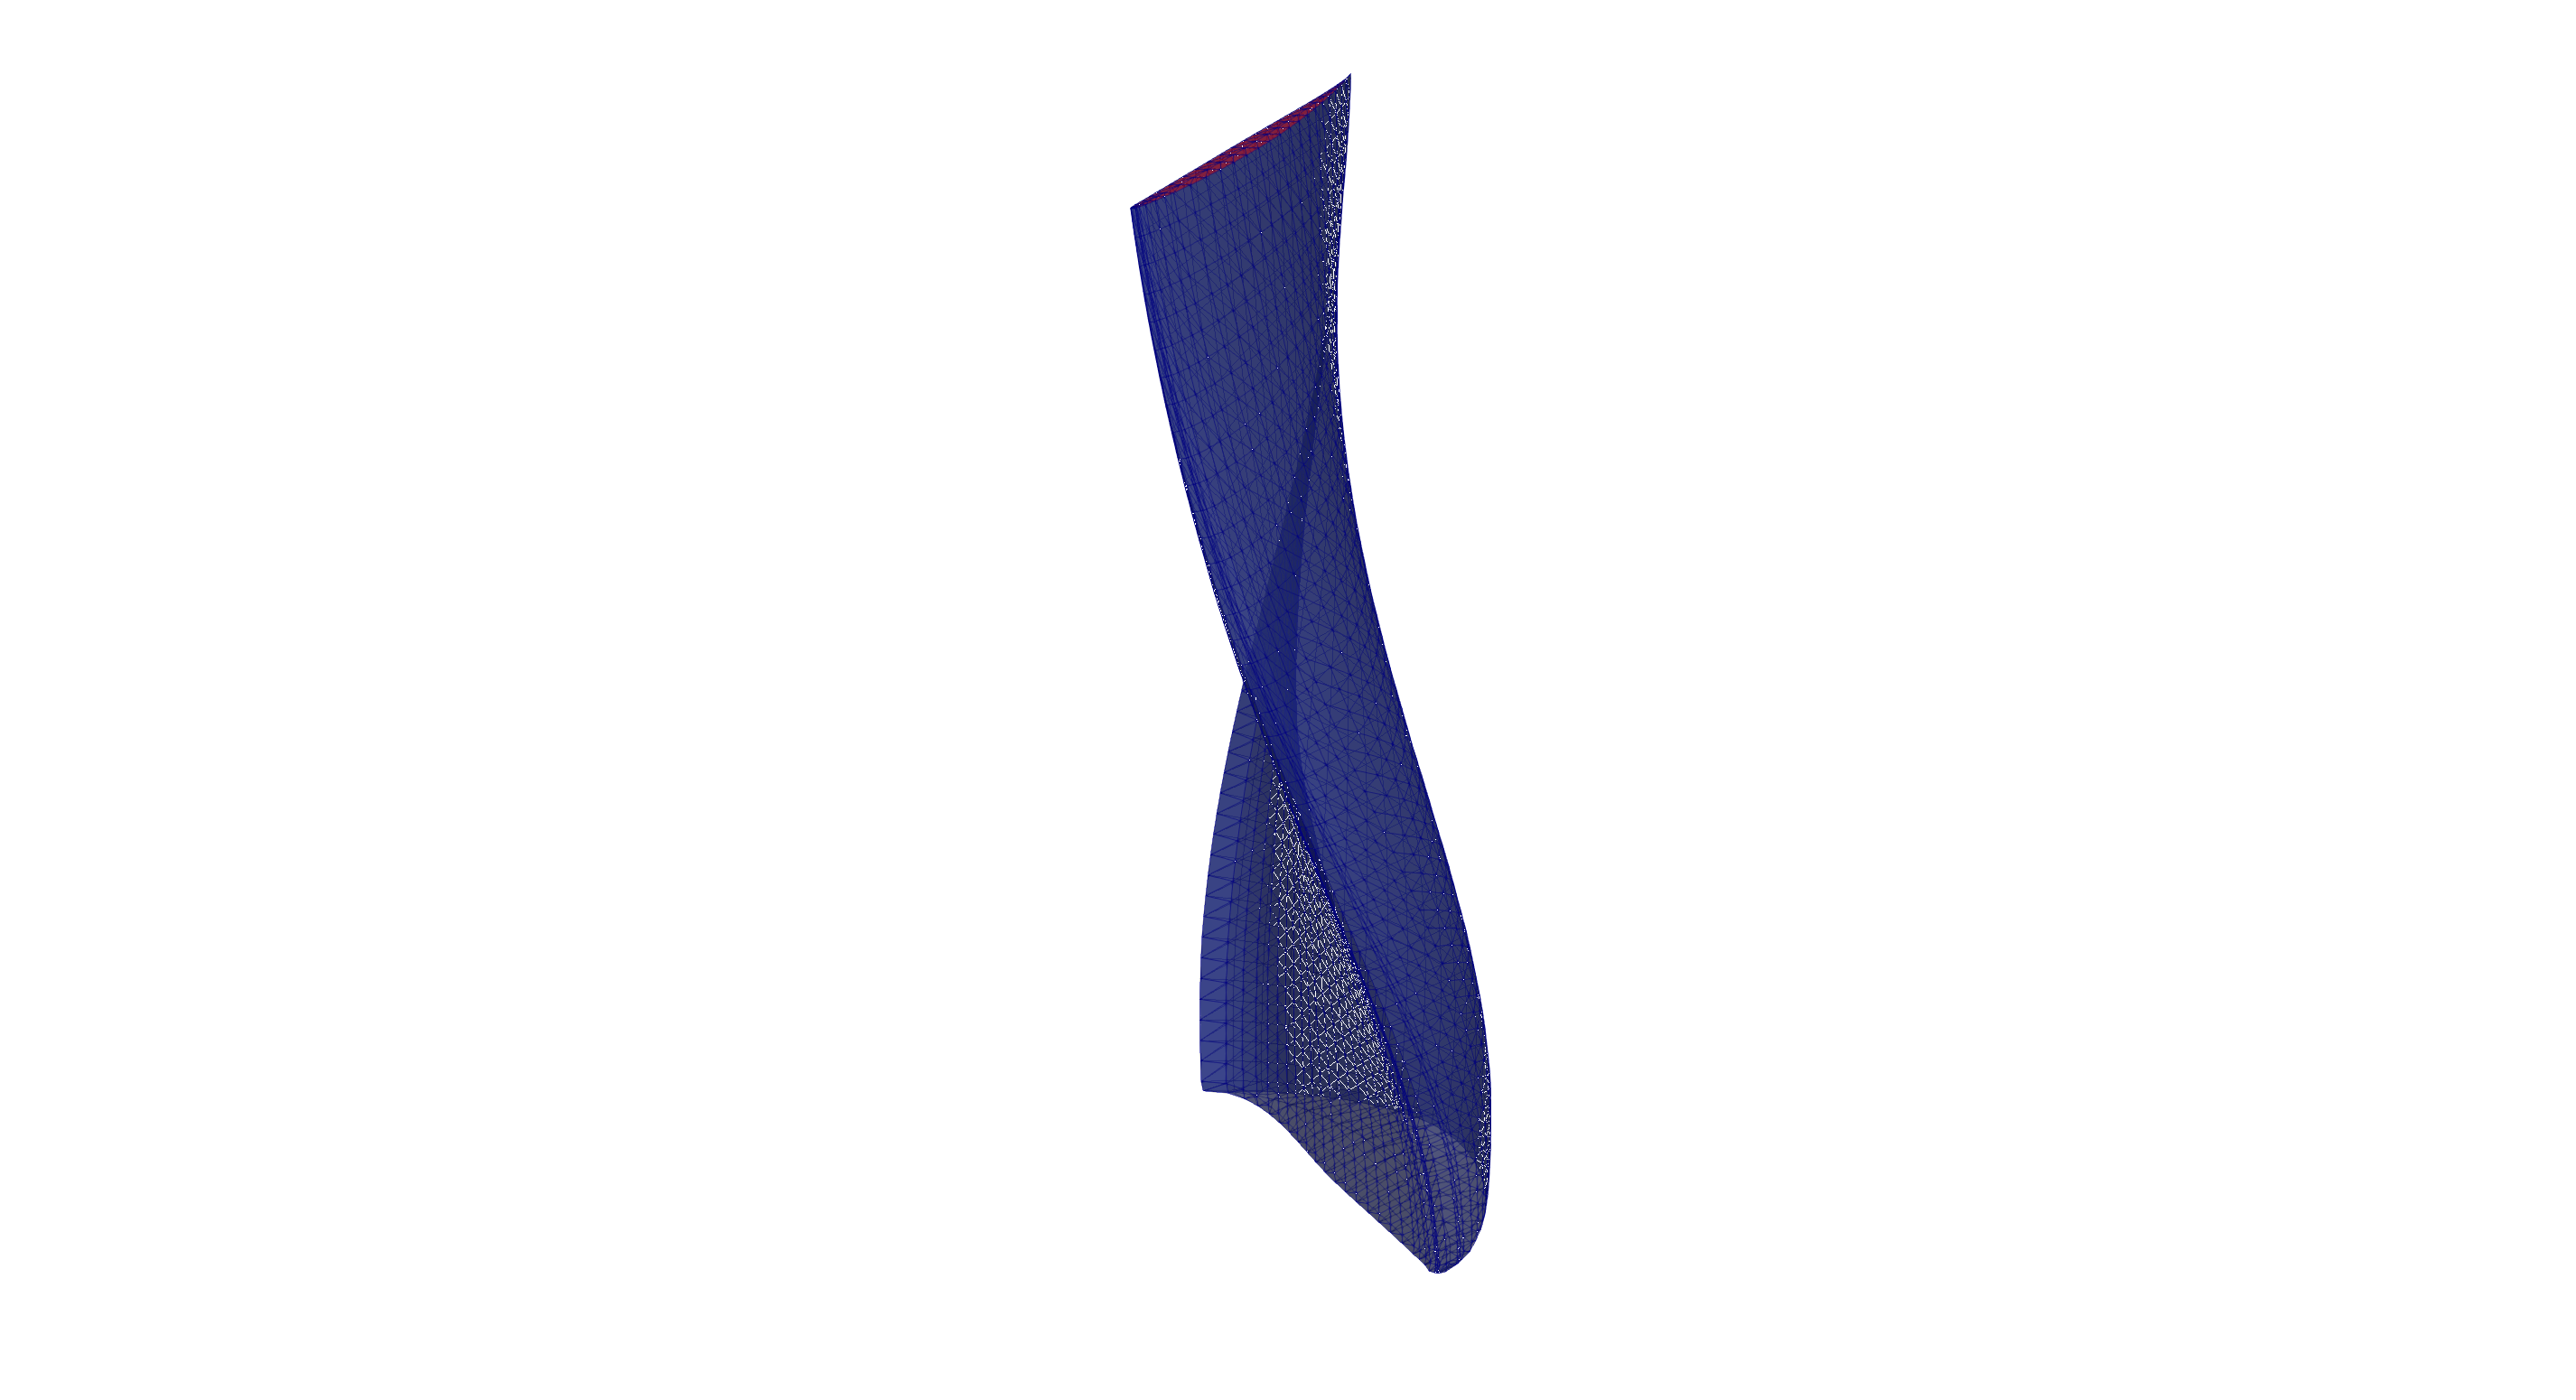
\includegraphics[width=1.5\textwidth]{figures/rotor.png}
					\caption{Rotor blade.}
				\end{figure}
			\column{0.5\textwidth}
				\begin{figure}
					\hspace{-2cm}
					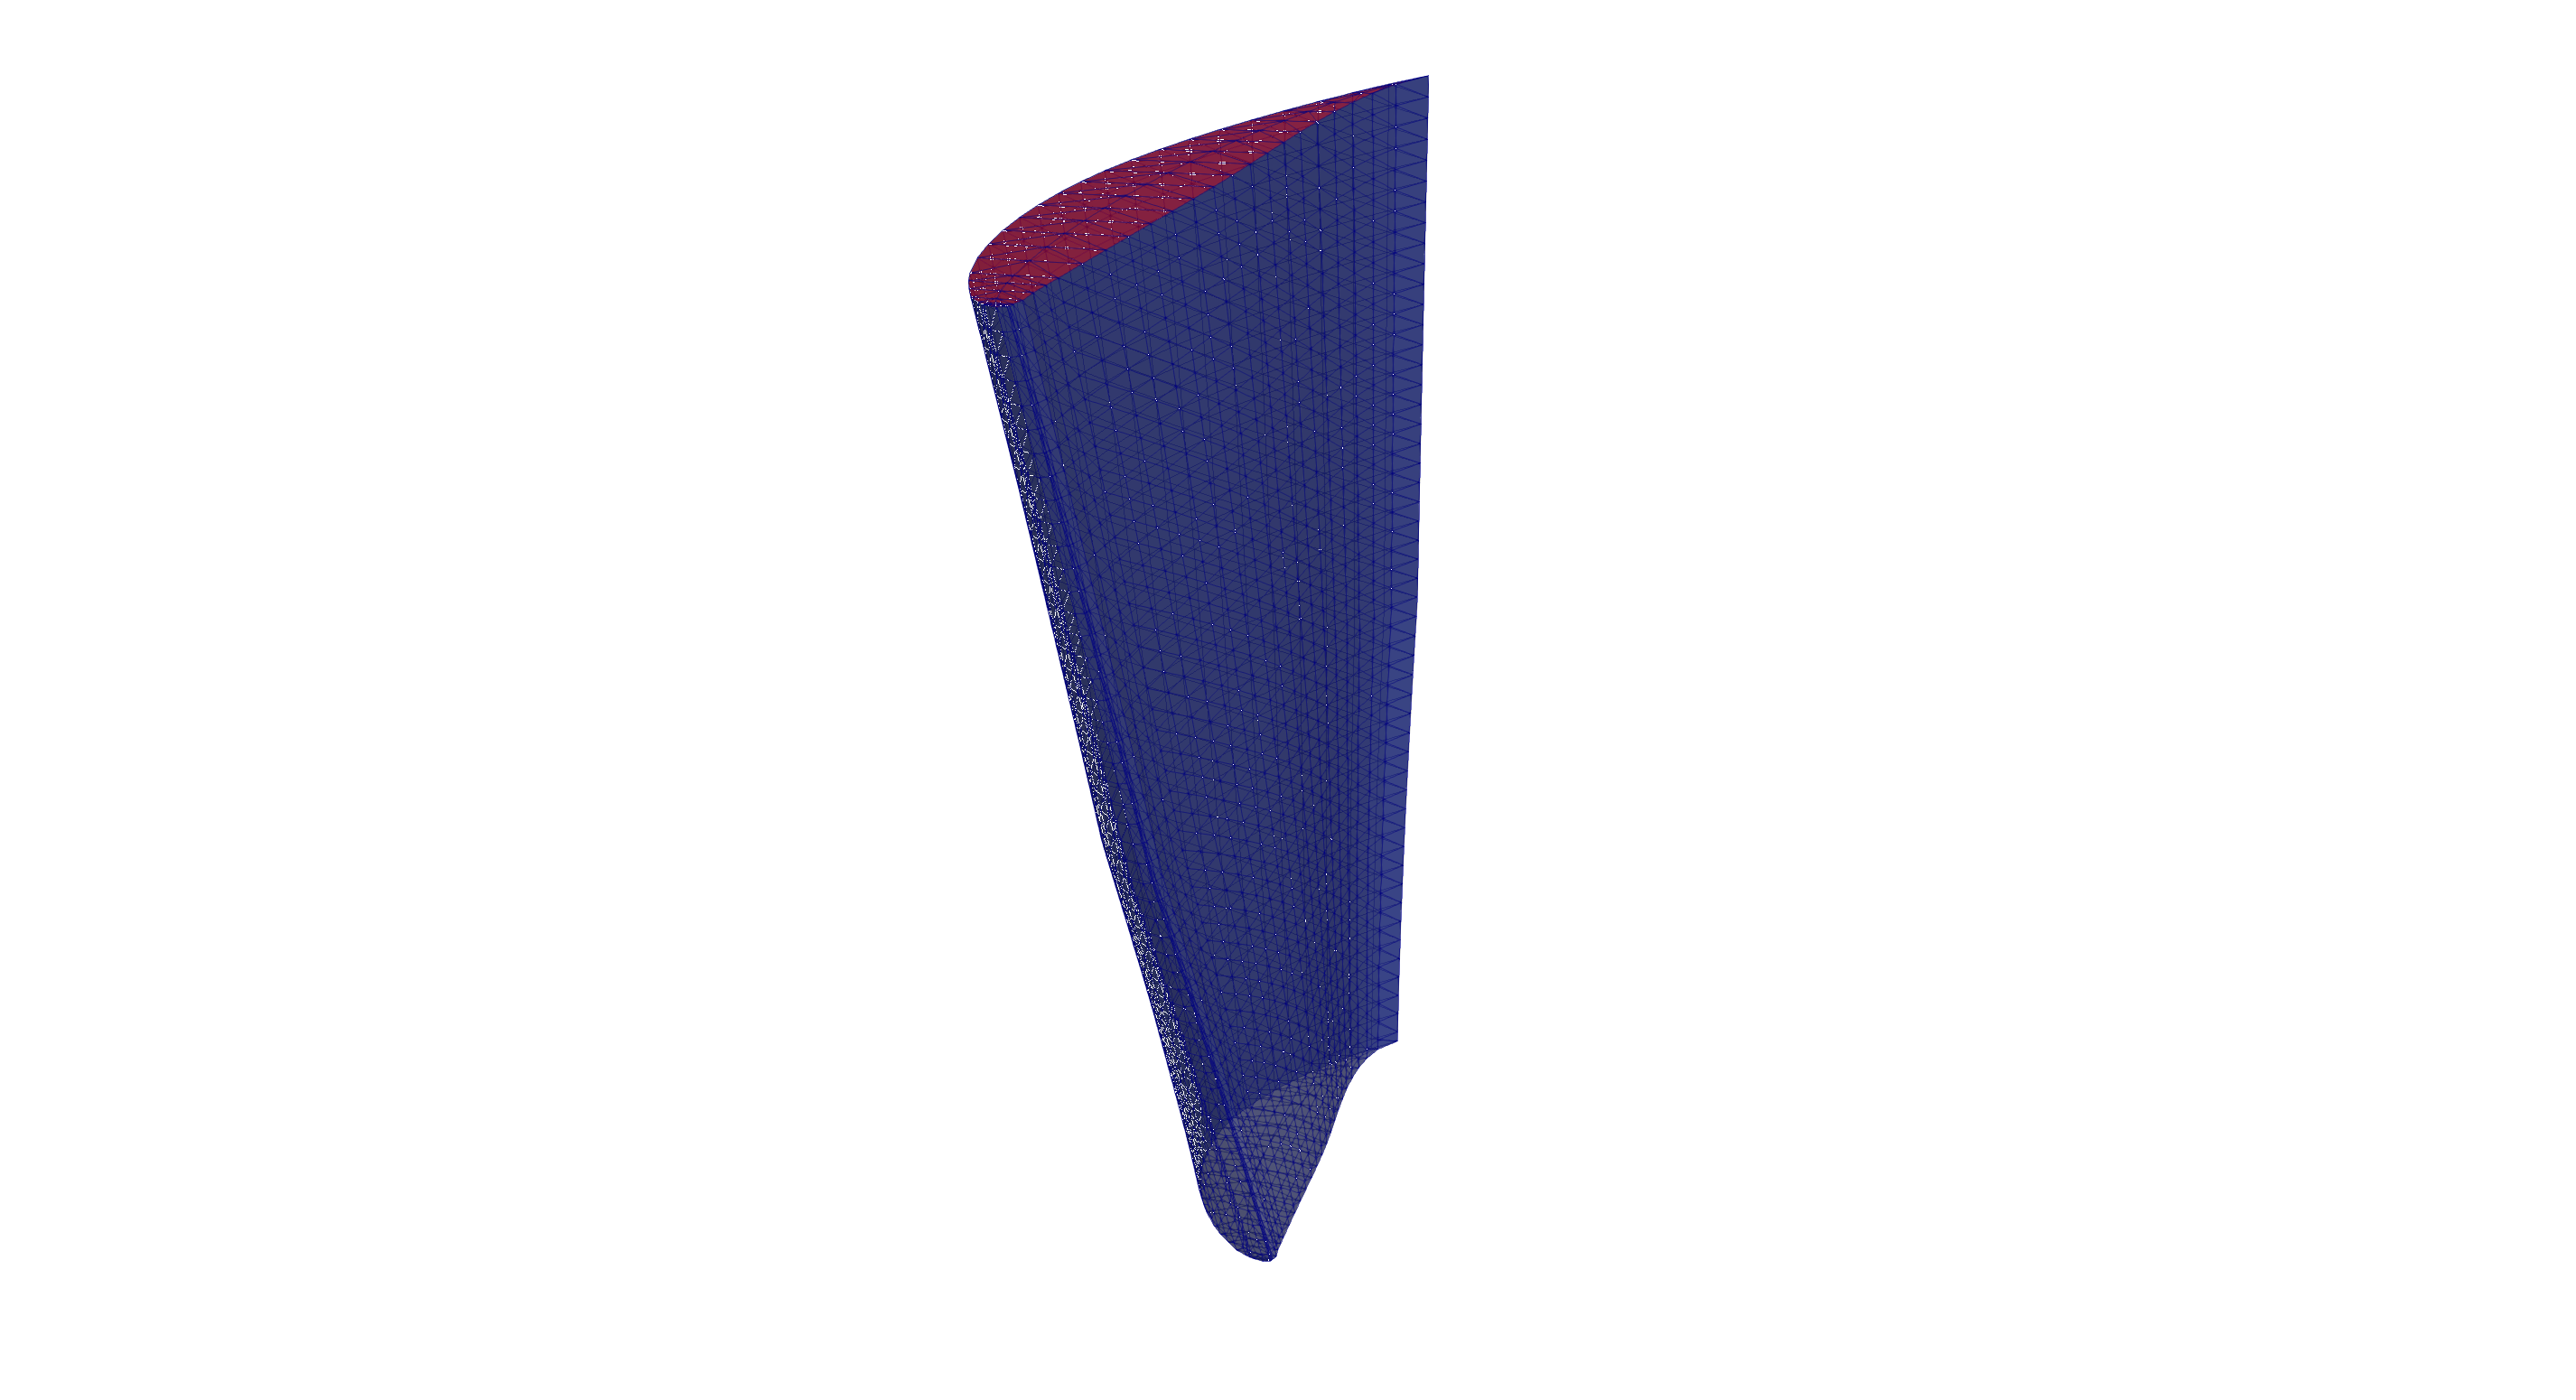
\includegraphics[width=1.5\textwidth]{figures/stator.png}
					\caption{Stator blade.}
				\end{figure}
		\end{columns}
	\end{frame}
	
	\begin{frame}{\textbf{Stage} plot}
		\begin{figure}
			\centering
			\includegraphics[width=1\textwidth]{figures/compressor.png}
		\end{figure}
	\end{frame}

\subsubsection{Efficiency}
	\begin{frame}[fragile]{Efficiency}
		The \textbf{rotor} efficiency is computed with:
		\begin{equation}
			\eta_{is_{rotor}} = \frac{W_1^2 - W_{2_{is}}^2}{W_1^2 - W_{2}^2} \nonumber 
		\end{equation}
		The \textbf{stator} efficiency is computed with:
		\begin{equation}
			\eta_{is_{stator}} = \frac{\Delta h_{is}}{\Delta h_{real}} \nonumber 
		\end{equation}
		The modeling results are stored into \verb|compressor_0.58_0.32_45_35.txt|.
	\end{frame}


	%\section{CFD}
	%\input{verification}
	    
	\begin{frame}[allowframebreaks]
		\printbibliography
	\end{frame}

	\begin{frame}
		\begin{center}
			{\Huge \emph {\textrm{Thank  ~you!}}}
		\end{center}
		
		\vspace{2cm}
		
		\Large{\textbf{Antonio Pucciarelli} \hfill 974675} \\ 
        
	\end{frame}
\end{document}
